\documentclass[conference]{IEEEtran}
\IEEEoverridecommandlockouts
\usepackage{cite}
\usepackage{amsmath,amssymb}
\usepackage{algorithm}
\usepackage{algpseudocode}
\usepackage{graphicx}
\usepackage{booktabs}
\usepackage{textcomp}
\usepackage{xcolor}
\usepackage{url}
\graphicspath{{figures/}}

\begin{document}

\title{Dynamic Timetable: Extracting Published College Timetables and Answering Natural-Language Questions with a Deterministic Compositional Query Planner}

\author{
\IEEEauthorblockN{Shivam Mulani}
\IEEEauthorblockA{\textit{Dept. of Computer Engineering}\\
\textit{Sardar Patel Institute of Technology}\\
Mumbai, India\\
UID 2024300141}
\and
\IEEEauthorblockN{Gurshaan Nandrajog}
\IEEEauthorblockA{\textit{Dept. of Computer Engineering}\\
\textit{Sardar Patel Institute of Technology}\\
Mumbai, India\\
UID 2024300146}
\and
\IEEEauthorblockN{Harshvarddhan Waghela}
\IEEEauthorblockA{\textit{Dept. of Computer Engineering}\\
\textit{Sardar Patel Institute of Technology}\\
Mumbai, India\\
UID 2024300272}
\and
\IEEEauthorblockN{Prof. Anant Nimkar}
\IEEEauthorblockA{\textit{Dept. of Computer Engineering}\\
\textit{Sardar Patel Institute of Technology}\\
Mumbai, India\\
(Project Guide)}
}

\maketitle

\begin{abstract}
College timetables are usually published as dense multi-page PDF grids that students and faculty
must read by hand. Such documents are hard for software too: lab cells stack several batches, subject
and faculty codes are expanded only in page-local legends, time labels are inconsistent, and names are
spelled differently across pages. This paper presents \emph{Dynamic Timetable}, a role-based system
that extracts the timetable as it is actually published (PDF, scanned image, spreadsheet or document),
detects scheduling clashes, and answers questions in plain English on Android, iOS and the web. We
contribute (i)~a constrained backtracking algorithm that resolves inconsistent time labels and accepts
a reading only when it is identical in every valid assignment, (ii)~a group-sort-sweep conflict detector
that separates intended overlaps from genuine clashes in $O(n\log n + m)$, and (iii)~a deterministic
\emph{compositional query planner} that maps a question to a typed plan of operation, filters, date
and time window and compiles it to parameterised SQL, so no SQL is ever generated from user text. On a
real 10-page Computer Engineering timetable the system verified 452 of 453 classes (99.8\%), reduced
542 raw overlaps to the 2 genuine clashes, answered questions with a median latency of 37--47\,ms, and
returned zero wrong answers under 32 concurrent clients. The full stack is open source and runs on a
free cloud tier.
\end{abstract}

\begin{IEEEkeywords}
timetable extraction, table recognition, natural language interface to databases, query planning,
interval scheduling, conflict detection, role-based access control, mobile applications
\end{IEEEkeywords}

\section{Introduction}
Every semester an engineering department publishes its timetable, typically as a PDF with one page per
class division. Students and faculty consult it several times a day to answer simple questions:
\emph{Where is my next class? Is room 508 free at 2\,pm? When is Prof.\ Nimkar free on Monday?} Answering
these by hand means locating the right page, row, column and lab batch, and then looking up abbreviations
in a legend at the bottom of the page. Clashes, such as one teacher in two rooms at once, are usually
discovered only when they happen, and old and revised versions of the PDF circulate together.

Two families of software address parts of this problem. Timetable \emph{generators} such as FET,
UniTime and aSc~\cite{fet,unitime,asc} solve the constraint problem of building a timetable, but they do
not read a timetable that has already been published by other means. Generic \emph{table extractors}
such as Tabula and Camelot~\cite{tabula,camelot} recover cell text but know nothing about lab batches,
legends or time rows. On the question-answering side, large language model (LLM) text-to-SQL systems
understand free text but can produce incorrect queries and are vulnerable to prompt and SQL
injection~\cite{greshake2023,pedro2023}, which is unacceptable when an answer decides where a student
walks next.

We present Dynamic Timetable, which starts from the published document and ends with exact answers.
The contributions of this paper are:
\begin{enumerate}
\item A timetable-aware extraction pipeline with page-local legend expansion, stacked lab-cell parsing,
      per-entry provenance and a constrained backtracking resolver for inconsistent time labels.
\item A conflict detector that distinguishes intended overlaps (parallel lab batches, elective options,
      combined sessions) from genuine teacher, room and batch clashes.
\item A deterministic compositional query planner over a closed vocabulary built from the timetable
      itself, with clarification instead of guessing and an explainable plan attached to every answer.
\item An evaluation on a real 10-page college timetable covering extraction quality, clash detection,
      latency, concurrency and test coverage.
\end{enumerate}

\section{Related Work}
\subsection{Automated timetabling}
University timetabling has been studied extensively as a constraint satisfaction and optimisation
problem~\cite{schaerf1999,burke2002,lewis2008}. These methods \emph{construct} timetables; our work is
complementary and operates on the timetable after publication, when its consumers need to query it and
administrators need to check it.

\subsection{Table recognition and OCR}
Table recognition from documents is a long-standing problem~\cite{zanibbi2004,kieninger1998}, with
benchmark competitions such as ICDAR 2013~\cite{gobel2013}. Tesseract~\cite{smith2007} is a widely used
open-source OCR engine. General-purpose extractors recover grids well but do not interpret domain
semantics; in a timetable, a single cell may encode four lab batches, each with its own teacher, subject
and room, and abbreviations are defined only in the legend of the same page.

\subsection{Natural language interfaces to databases}
Natural language interfaces to databases (NLIDB) have a long history~\cite{androutsopoulos1995}. Neural
text-to-SQL models such as Seq2SQL~\cite{zhong2017} and benchmarks such as Spider~\cite{yu2018} have
greatly widened coverage, and LLMs extend it further. However, LLM-integrated applications are exposed
to indirect prompt injection~\cite{greshake2023} and prompt-to-SQL injection~\cite{pedro2023}, and their
outputs are not reproducible. For a narrow, high-stakes domain we instead adopt a deterministic planner
over a closed vocabulary that compiles only to pre-written parameterised templates.

\subsection{Temporal reasoning and access control}
Clash detection rests on interval relations~\cite{allen1983}; we use the end-exclusive overlap
predicate $a.s < b.e \wedge b.s < a.e$ with sorting and sweeping~\cite{cormen2009}. Access is governed by
role-based access control (RBAC)~\cite{sandhu1996}, with credentials hashed by Argon2id~\cite{biryukov2016}
and sessions carried in JSON Web Tokens~\cite{rfc7519}, following OWASP guidance~\cite{owasp2021}.

\section{System Architecture}
Fig.~\ref{fig:arch} shows the architecture. A single React Native code base built with
Expo~\cite{reactnative,expo} serves Android, iOS and the web. It communicates over HTTPS with a REST
API~\cite{fielding2000} implemented in FastAPI~\cite{fastapi}. All state lives in PostgreSQL
16~\cite{postgresdocs}: 31 tables in third normal form~\cite{codd1970,silberschatz2019}, created by three
Alembic migrations. Uploads are processed asynchronously: the upload transaction inserts a job row, and
a worker claims it with \texttt{SELECT \ldots{} FOR UPDATE SKIP LOCKED}, a producer--consumer pattern
that needs no separate message broker. The system deploys from a single blueprint file and Docker image
to a free platform-as-a-service tier~\cite{render}.

\begin{figure}[t]
\centering
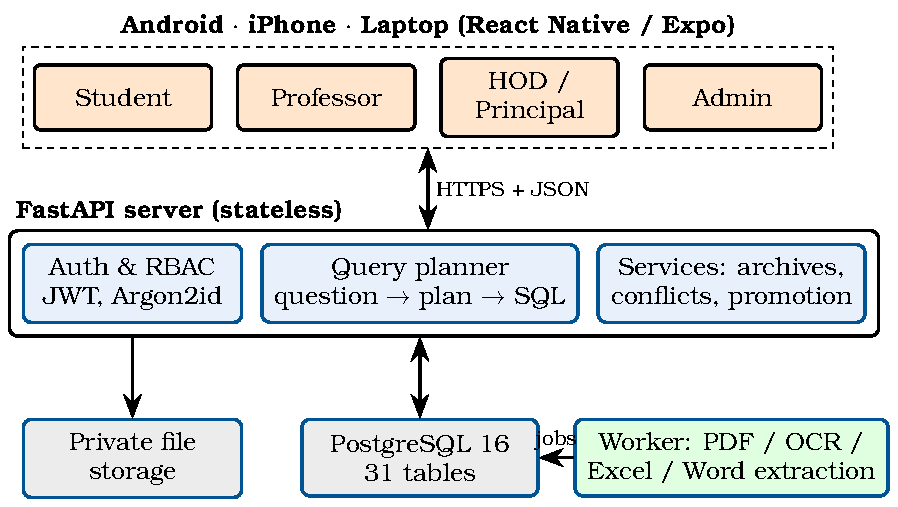
\includegraphics[width=\columnwidth]{arch.pdf}
\caption{System architecture: one cross-platform client, a FastAPI back end with a background worker,
and PostgreSQL as both database and job queue.}
\label{fig:arch}
\end{figure}

Business rules are enforced in the schema where possible: \texttt{CHECK} constraints on day of week,
\texttt{end\,>\,start}, confidence in $[0,1]$ and allowed verification states; partial unique indexes for
one current academic placement per student and idempotent uploads; and composite foreign keys
\texttt{(timetable\_id, owner\_user\_id)} so that a user can reference only their own personal timetable.
Each extracted entry retains its raw text, source page and confidence for review.

\section{Extraction Pipeline}
Fig.~\ref{fig:pipe} summarises the pipeline. PyMuPDF~\cite{pymupdf} supplies words with coordinates and
the ruled lines of the page; scanned pages are passed through Tesseract. Lines are clustered into rows
and columns to recover the grid, the day and time headers are located, and each cell is parsed.

\begin{figure*}[t]
\centering
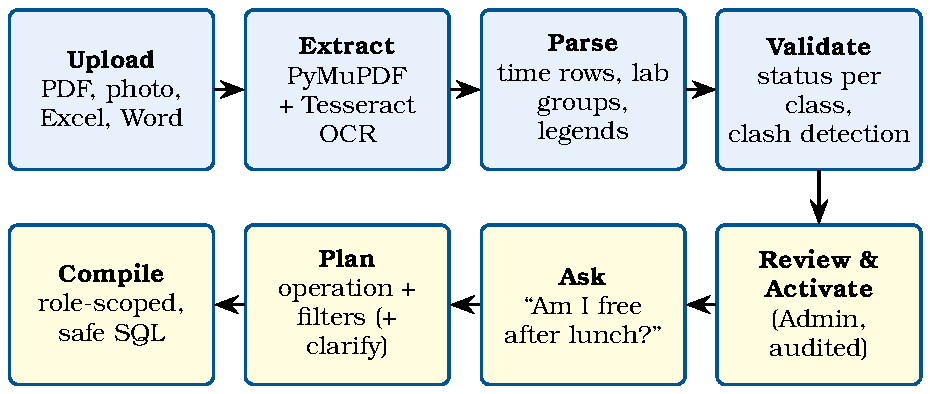
\includegraphics[width=0.62\textwidth]{pipe.pdf}
\caption{Extraction pipeline from upload to a verified, published timetable.}
\label{fig:pipe}
\end{figure*}

\subsection{Cell parsing and legends}
A cell is split into lines, and lines belonging to one lab sub-group (e.g.\ \texttt{A1 COA Lab JS 606-4})
are grouped. Within a group, a batch token matches \texttt{[A-D][1-4]}, the room is the last token
matching a room pattern, faculty codes are tokens present in the page legend, and the remainder is the
subject. Codes are expanded \emph{only} if they appear in the legend of the same page; otherwise the code
is kept and an informational flag is raised. Each entry is then validated into one of
\textsc{Verified}, \textsc{Unverified}, \textsc{Incomplete} or \textsc{Rejected}.

\subsection{Time-row resolution by constrained backtracking}
Printed time labels are unreliable. The real document labels the noon row ``12.15 a.m.\ to 01.15 p.m.''
and many labels omit a.m./p.m.\ altogether. Algorithm~\ref{alg:time} converts each label into a small set
of plausible intervals (between 07:00 and 21:00, at most six hours long) and enumerates assignments in
which no row starts before the previous row ends. A reading is marked \emph{certain} only if it is the
same in every valid assignment; otherwise the row is flagged for review rather than guessed. The noon row
is therefore accepted as 12:15--13:15 because its neighbours end at 12:15 and start at 13:15, not because
the rule assumes it.

\begin{algorithm}[t]
\caption{Resolve a column of time labels}\label{alg:time}
\begin{algorithmic}[1]
\Require labels $L_1..L_r$ from top to bottom
\Ensure per row: interval and certainty, or a review flag
\For{$i \gets 1$ \textbf{to} $r$}
  \State $O_i \gets$ plausible readings $(s,e)$ of $L_i$
  \If{$O_i=\emptyset$} $O_i \gets$ non-literal readings \EndIf
\EndFor
\State $S \gets \emptyset$
\Procedure{Walk}{$i, p, A$}
  \If{$|S| > 64$} \Return \EndIf
  \If{$i > r$} $S \gets S \cup \{A\}$; \Return \EndIf
  \ForAll{$(s,e)\in O_i$ \textbf{with} $s \ge p$}
     \State \Call{Walk}{$i+1, e, A\cdot(s,e)$}
  \EndFor
\EndProcedure
\State \Call{Walk}{$1, 0, \langle\rangle$}
\For{$i \gets 1$ \textbf{to} $r$}
  \State $R_i \gets \{A_i : A \in S\}$
  \If{$|R_i|=1$ and literal} row $i$ is \textsc{Certain}
  \ElsIf{$|R_i|=1$} keep, flag \texttt{TIME\_LABEL\_INCONSISTENT}
  \Else{} leave empty, flag \texttt{TIME\_AMBIGUOUS\_AMPM}
  \EndIf
\EndFor
\end{algorithmic}
\end{algorithm}

Because the search is bounded at 64 complete assignments, its cost is $O(64r)$ for $r$ rows, negligible
compared with page rendering.

\section{Conflict Detection}
A naive pairwise check is both slow, $O(n^2)$, and noisy, because timetables contain many \emph{intended}
overlaps. Algorithm~\ref{alg:conflict} groups entries by resource (teacher, room or batch) and day, sorts
each group by start time, and sweeps forward, stopping as soon as a later entry starts after the current
one ends. A pair is reported only if the intervals overlap and the overlap is not intended: entries from
the same source cell, the same combined session printed on several pages, parallel elective options, or a
sub-group's own written period. The total cost is $O(n\log n + m)$ for $m$ reported pairs. A clash is
\textsc{Confirmed} when both entries are verified, mapped to master data and time-certain, and
\textsc{Possible} otherwise.

\begin{algorithm}[t]
\caption{Group, sort and sweep}\label{alg:conflict}
\begin{algorithmic}[1]
\Require entries $E$ with day and times
\State $G \gets$ hash map from (resource, key, day) to lists
\ForAll{$x\in E$, resource $(k,\mathit{key})$ of $x$}
  \State append $x$ to $G[(k,\mathit{key},x.\mathit{day})]$
\EndFor
\ForAll{group $g\in G$}
  \State sort $g$ by start
  \For{$i\gets 1$ \textbf{to} $|g|$}
    \For{$j\gets i+1$ \textbf{to} $|g|$}
      \If{$g_j.s \ge g_i.e$} \textbf{break} \EndIf
      \If{\textbf{not} \textsc{Intended}$(g_i,g_j)$} report $(k,g_i,g_j)$ \EndIf
    \EndFor
  \EndFor
\EndFor
\end{algorithmic}
\end{algorithm}

\section{Compositional Query Planner}
\subsection{From fixed intents to composed plans}
An initial design mapped each question to one of about thirty fixed intents. This limited users to
questions the designers had anticipated. The final design instead recognises \emph{independent pieces}
of a question and composes them into a typed plan:
\begin{itemize}
\item \textbf{Operation}: \textsc{List}, \textsc{Count}, \textsc{Exists}, \textsc{Total\_Hours},
      \textsc{First}, \textsc{Last}, \textsc{Next}, \textsc{Per\_Day}, \textsc{Span},
      \textsc{Free\_Slots}, \textsc{Breaks}, \textsc{After\_Course}, \textsc{Before\_Course},
      \textsc{Teachers}, \textsc{Per\_Room}, \textsc{Room\_Info}, \textsc{Conflicts} (17 in total).
\item \textbf{Filters}: the asking user, a batch, a professor, a room, a course; lab or lecture; room type.
\item \textbf{When}: a date, a weekday, this or next week, or the whole weekly timetable.
\item \textbf{Time window}: at, after, before, between, after lunch, or now.
\item \textbf{Metric and sort} for day-wise questions: most or least classes or hours, earliest or latest
      start or finish.
\end{itemize}
For example, ``Which day do I finish earliest?'' becomes
\texttt{\{op: PER\_DAY, filters: me, metric: LAST\_END, sort: EARLIEST\}}, and ``How many labs do I have this
week?'' becomes \texttt{\{op: COUNT, kind: LAB, when: \{week: this\}\}}. Questions needing dedicated logic
(free rooms, a professor's free time, archives) keep specialised templates; all other plans are compiled
by one composed executor from shared building blocks.

\subsection{Vocabulary and name resolution}
Entities are recognised by scanning the question against a vocabulary built from the active timetable
itself (about 200 labels for the real document): teacher names and codes, rooms, subjects and batches.
Teachers can be referred to by code, first name, surname or ``\emph{X} sir/ma'am''; entries that share a
faculty code are merged, which reconciles spelling variants such as ``Sushama'' and ``Sushma''. Subjects
match on partial words and on words within edit distance one, which handles the document's own typo
``Discreate''. A lab batch such as A2 also includes the lectures of its parent division. Resolution
proceeds from exact match to unique word match to fuzzy \emph{suggestions}; the system never silently
chooses among several candidates.

\subsection{Safety and explainability}
Every plan is validated against a closed, immutable registry of operations and parameter values before
execution, and is compiled into pre-written parameterised SQL. User text never reaches the SQL string, so
injection is not possible by construction. When a question is genuinely ambiguous, for example ``at 2''
(a.m.\ or p.m.) or a surname shared by two teachers, the engine returns a clarification request instead of
an answer. Each answer carries its plan in a \texttt{meta.plan} field that the app can display, making the
result auditable.

\subsection{Access policy}
The official timetable is public information within the college, so any authenticated user may view any
teacher's, batch's or room's schedule and ask questions about it. Personal timetables are private to
their owner; requesting another user's personal timetable returns \texttt{404}. Clash reports are visible to
the HOD, Principal and Admin, and only the Admin may upload, correct or publish. Access tokens are valid for
15 minutes; refresh tokens rotate, are stored only as hashes, and reuse of a revoked token revokes the
whole token family.

\section{Implementation}
The back end comprises about 10.5k lines of Python 3.13 with SQLAlchemy 2 and Alembic; the client
comprises about 5.5k lines of strict TypeScript using Expo Router and TanStack Query. The client performs a
single-flight token refresh: the first \texttt{401} triggers one refresh call and other failing requests
wait for it. Fig.~\ref{fig:screens} shows representative screens: the student home and day view, the Ask
screen with composed answers, the timetable picker for viewing any teacher, batch or room, and the
administration views.

\begin{figure*}[t]
\centering
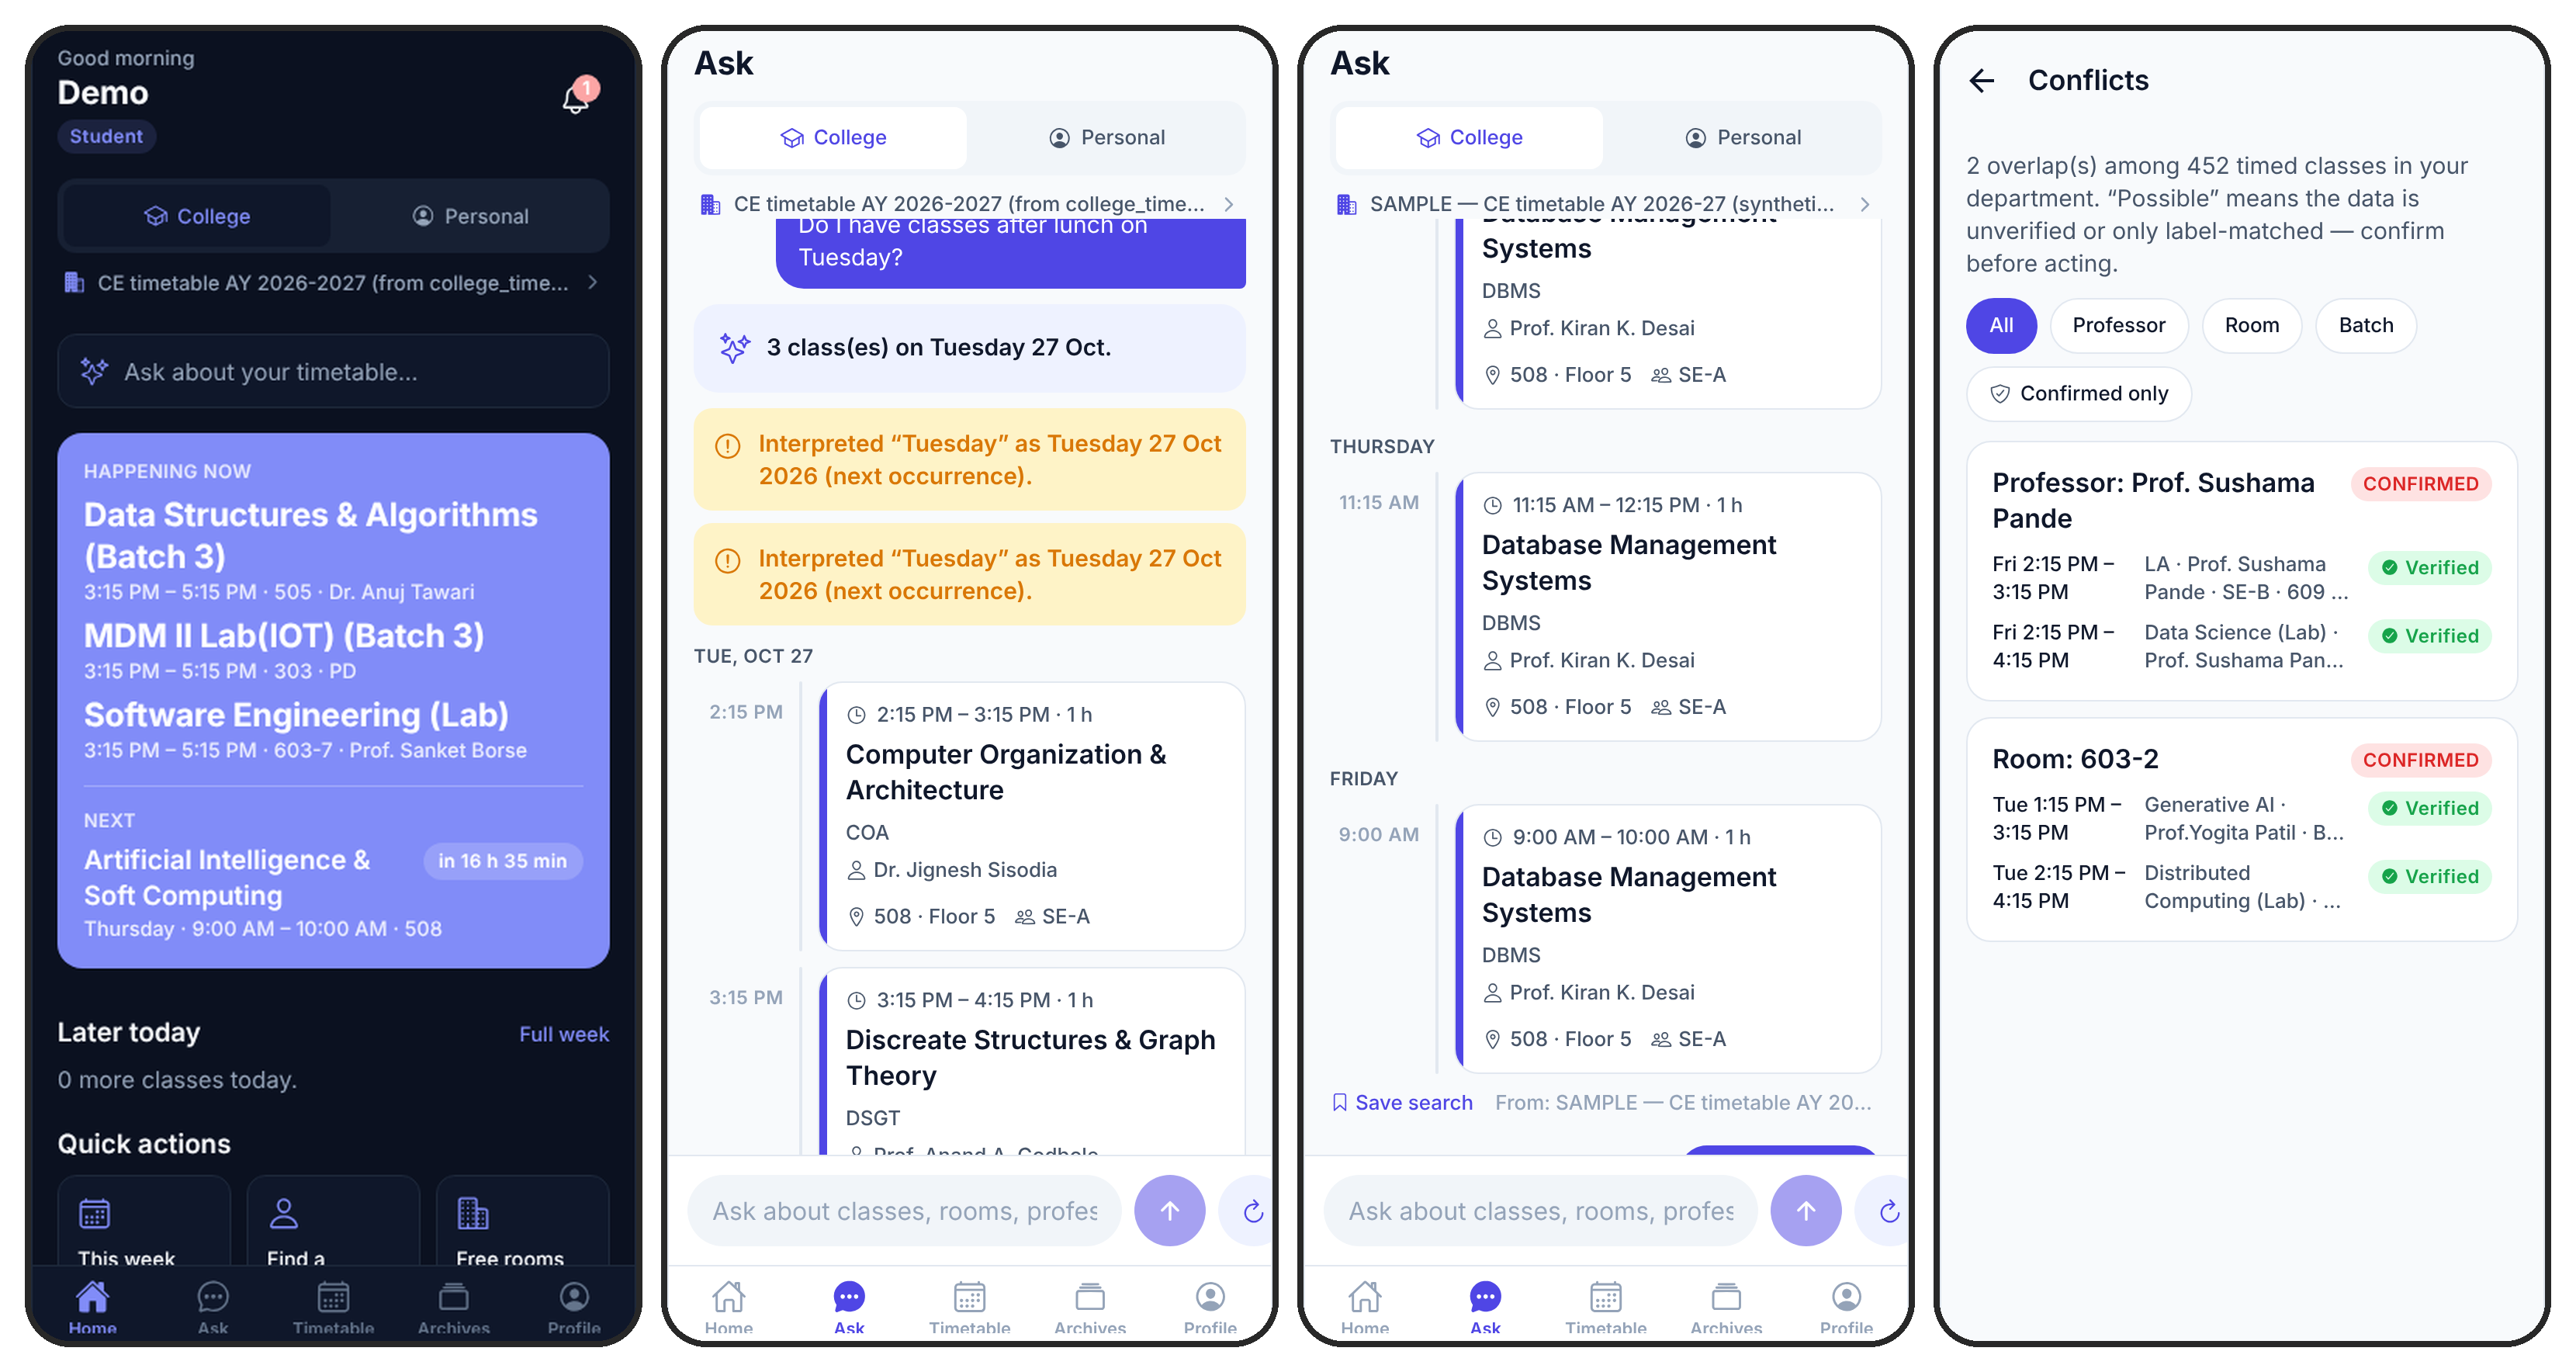
\includegraphics[width=\textwidth]{screens.png}
\caption{Representative screens of the mobile and web client.}
\label{fig:screens}
\end{figure*}

\section{Evaluation}
\subsection{Setup}
All measurements use the department's real 10-page Computer Engineering timetable (SE, TE, BE and
M.Tech.\ divisions). Performance was measured on a Linux VM with 4 vCPU and 15\,GB RAM, with PostgreSQL 16
on the same machine and four API worker processes.

\subsection{Extraction quality}
The pipeline produced 570 rows: 453 classes plus breaks and activities. Of the 453 classes, 452 were
\textsc{Verified} (99.8\%) and one was \textsc{Incomplete}, an M.Tech.\ row with no printed time, which the
system flagged rather than guessed. The whole document was processed in 1.65\,s (five runs: 1.64--1.72\,s),
about 0.17\,s per page, with a peak memory of 82\,MB.

\subsection{Conflict detection}
A naive pairwise check reported 542 overlaps. Adding the same-cell and lab-batch rules reduced this to 25,
and adding elective and combined-session rules reduced it to 2. Both remaining clashes were confirmed by
hand against the PDF, giving zero false reports on this document (Table~\ref{tab:clash}).

\begin{table}[t]
\centering
\caption{Effect of intended-overlap rules on reported clashes}
\label{tab:clash}
\begin{tabular}{@{}lr@{}}
\toprule
\textbf{Rule set} & \textbf{Reported}\\
\midrule
Naive pairwise overlap & 542\\
+ same source cell, parallel lab batches & 25\\
+ elective options, combined sessions & 2\\
\midrule
Genuine clashes (manual check) & 2\\
\bottomrule
\end{tabular}
\end{table}

\subsection{Latency and concurrency}
Table~\ref{tab:latency} reports single-user latency over 50 requests per question type: medians of
37--47\,ms and 95th percentiles of at most 54\,ms, well below the 300\,ms objective. Eliminating N+1 queries
by eager loading halved the SQL statements per search from about 50 to 25.

\begin{table}[t]
\centering
\caption{Single-user latency per question type (ms)}
\label{tab:latency}
\setlength{\tabcolsep}{4pt}
\begin{tabular}{@{}lrr@{}}
\toprule
\textbf{Question} & \textbf{p50} & \textbf{p95}\\
\midrule
What is my next class? & 42 & 52\\
What are my classes on Monday? & 44 & 52\\
Find all DBMS classes & 45 & 51\\
Do I have classes after lunch on Tuesday? & 47 & 54\\
(Professor) What is my schedule on Monday? & 37 & 46\\
Which rooms are free at 10 am today? & 43 & 51\\
Show the schedule of room 508 on Monday & 41 & 49\\
\bottomrule
\end{tabular}
\end{table}

For the load test, $N$ concurrent clients, each logged in as a different real student account, sent 30
back-to-back requests cycling through five realistic questions, and every response was checked for
correctness. Table~\ref{tab:load} shows that throughput peaks at about 60 requests per second at eight
clients; beyond that, requests queue and latency grows, but no request failed and no answer was wrong even
at 32 clients. The API worker used 113--116\,MB of memory and the database occupied 12\,MB.

\begin{table}[t]
\centering
\caption{Load test with increasing concurrent clients}
\label{tab:load}
\begin{tabular}{@{}rrrrr@{}}
\toprule
\textbf{Clients} & \textbf{Wrong} & \textbf{req/s} & \textbf{p50 (ms)} & \textbf{p95 (ms)}\\
\midrule
1 & 0 & 18.6 & 49 & 57\\
2 & 0 & 25.4 & 75 & 90\\
4 & 0 & 46.5 & 64 & 90\\
8 & 0 & 60.4 & 90 & 141\\
16 & 0 & 54.1 & 183 & 354\\
32 & 0 & 57.4 & 410 & 635\\
\bottomrule
\end{tabular}
\end{table}

\subsection{Testing}
The back end has 179 automated tests run against a real PostgreSQL instance, covering the query engine
(59), the real college timetable (33), extraction (24), authentication and token rotation (15), a reference
PDF (14), administration (13), uploads and privacy isolation (13) and deployment (8). The client has 20
Jest tests and compiles under strict TypeScript, and 45 end-to-end checks exercise the running API. All
pass.

\subsection{Comparison}
Table~\ref{tab:compare} compares the system with existing approaches. It is the only option that reads
the published document and also answers questions with reproducible, injection-safe results.

\begin{table}[t]
\centering
\caption{Comparison with existing approaches}
\label{tab:compare}
\setlength{\tabcolsep}{2pt}
\footnotesize
\begin{tabular}{@{}lccccc@{}}
\toprule
\textbf{Criterion} & \textbf{Manual} & \textbf{FET/aSc} & \textbf{Tabula} & \textbf{LLM} & \textbf{Ours}\\
\midrule
Reads published PDF & -- & No & Partly & No & Yes\\
Labs and legends & Human & Yes & No & Depends & Yes\\
Plain-English questions & No & No & No & Yes & Yes\\
Reproducible, injection-safe & -- & -- & -- & No & Yes\\
Clash check after publishing & No & At creation & No & No & Yes\\
Cost & Free & Free/Paid & Free & Paid API & Free\\
\bottomrule
\end{tabular}
\end{table}

\section{Discussion and Limitations}
The deterministic planner trades open-ended coverage for exactness: a phrasing outside the vocabulary
yields a clarification or a suggestion rather than a confident wrong answer. In this domain we consider
that the right trade-off. Several limitations remain. Extraction accuracy was assessed by verification
status and manual checks, not by precision and recall against independently hand-labelled pages. The load
test ran on development hardware, not on the free production instance. Some short forms (for example
``AI'' for an elective) are not yet recognised, and a bare time such as ``at 2'' always triggers an
a.m./p.m.\ clarification. Store builds and push notifications have not yet been released.

\section{Conclusion and Future Work}
Dynamic Timetable shows that a published, irregular timetable PDF can be turned into a reliable,
queryable service without manual data entry. Constrained backtracking resolves inconsistent time labels
with provable certainty, a group-sort-sweep detector isolates the genuine clashes among hundreds of
intended overlaps, and a deterministic compositional planner answers a wide range of plain-English
questions in tens of milliseconds while remaining explainable and injection-safe. Future work includes
measuring per-field precision and recall on hand-labelled pages, college single sign-on, change alerts
sent only to affected users, an optional LLM that \emph{suggests} plans which must still pass the same
validator, and capacity testing on production hardware.

\section*{Acknowledgment}
The authors thank Prof.\ Anant Nimkar for his guidance and Dr.\ Sudhir Dhage, Head of the Department of
Computer Engineering, Sardar Patel Institute of Technology, for his support.

\begin{thebibliography}{99}

\bibitem{fet}
L.~Lalescu \emph{et al.}, ``FET -- Free Timetabling Software.'' [Online]. Available:
https://lalescu.ro/liviu/fet/

\bibitem{unitime}
UniTime, ``UniTime -- Comprehensive University Timetabling System.'' [Online]. Available:
https://www.unitime.org/

\bibitem{asc}
Applied Software Consultants, ``aSc Timetables.'' [Online]. Available: https://www.asctimetables.com/

\bibitem{tabula}
Tabula, ``Tabula: Extract tables from PDFs.'' [Online]. Available: https://tabula.technology/

\bibitem{camelot}
Camelot, ``Camelot: PDF table extraction for humans.'' [Online]. Available:
https://camelot-py.readthedocs.io/

\bibitem{greshake2023}
K.~Greshake, S.~Abdelnabi, S.~Mishra, C.~Endres, T.~Holz and M.~Fritz, ``Not what you've signed up
for: Compromising real-world LLM-integrated applications with indirect prompt injection,'' in
\emph{Proc. 16th ACM Workshop on Artificial Intelligence and Security (AISec)}, 2023, pp.~79--90.

\bibitem{pedro2023}
R.~Pedro, D.~Castro, P.~Carreira and N.~Santos, ``From prompt injections to SQL injection attacks:
How protected is your LLM-integrated web application?,'' \emph{arXiv preprint arXiv:2308.01990}, 2023.

\bibitem{schaerf1999}
A.~Schaerf, ``A survey of automated timetabling,'' \emph{Artificial Intelligence Review}, vol.~13,
no.~2, pp.~87--127, 1999.

\bibitem{burke2002}
E.~K. Burke and S.~Petrovic, ``Recent research directions in automated timetabling,''
\emph{European Journal of Operational Research}, vol.~140, no.~2, pp.~266--280, 2002.

\bibitem{lewis2008}
R.~Lewis, ``A survey of metaheuristic-based techniques for university timetabling problems,''
\emph{OR Spectrum}, vol.~30, no.~1, pp.~167--190, 2008.

\bibitem{zanibbi2004}
R.~Zanibbi, D.~Blostein and J.~R. Cordy, ``A survey of table recognition: Models, observations,
transformations, and inferences,'' \emph{International Journal on Document Analysis and Recognition},
vol.~7, no.~1, pp.~1--16, 2004.

\bibitem{kieninger1998}
T.~Kieninger and A.~Dengel, ``The T-Recs table recognition and analysis system,'' in
\emph{Document Analysis Systems: Theory and Practice (DAS'98)}, LNCS vol.~1655, Springer, 1999,
pp.~255--270.

\bibitem{gobel2013}
M.~G\"obel, T.~Hassan, E.~Oro and G.~Orsi, ``ICDAR 2013 table competition,'' in \emph{Proc. 12th
International Conference on Document Analysis and Recognition (ICDAR)}, 2013, pp.~1449--1453.

\bibitem{smith2007}
R.~Smith, ``An overview of the Tesseract OCR engine,'' in \emph{Proc. 9th International Conference on
Document Analysis and Recognition (ICDAR)}, 2007, pp.~629--633.

\bibitem{androutsopoulos1995}
I.~Androutsopoulos, G.~D. Ritchie and P.~Thanisch, ``Natural language interfaces to databases --
an introduction,'' \emph{Natural Language Engineering}, vol.~1, no.~1, pp.~29--81, 1995.

\bibitem{zhong2017}
V.~Zhong, C.~Xiong and R.~Socher, ``Seq2SQL: Generating structured queries from natural language
using reinforcement learning,'' \emph{arXiv preprint arXiv:1709.00103}, 2017.

\bibitem{yu2018}
T.~Yu \emph{et al.}, ``Spider: A large-scale human-labeled dataset for complex and cross-domain
semantic parsing and text-to-SQL task,'' in \emph{Proc. Conference on Empirical Methods in Natural
Language Processing (EMNLP)}, 2018, pp.~3911--3921.

\bibitem{allen1983}
J.~F. Allen, ``Maintaining knowledge about temporal intervals,'' \emph{Communications of the ACM},
vol.~26, no.~11, pp.~832--843, 1983.

\bibitem{cormen2009}
T.~H. Cormen, C.~E. Leiserson, R.~L. Rivest and C.~Stein, \emph{Introduction to Algorithms},
3rd~ed. Cambridge, MA: MIT Press, 2009.

\bibitem{sandhu1996}
R.~S. Sandhu, E.~J. Coyne, H.~L. Feinstein and C.~E. Youman, ``Role-based access control models,''
\emph{IEEE Computer}, vol.~29, no.~2, pp.~38--47, 1996.

\bibitem{biryukov2016}
A.~Biryukov, D.~Dinu and D.~Khovratovich, ``Argon2: New generation of memory-hard functions for
password hashing and other applications,'' in \emph{Proc. IEEE European Symposium on Security and
Privacy (EuroS\&P)}, 2016, pp.~292--302.

\bibitem{rfc7519}
M.~Jones, J.~Bradley and N.~Sakimura, ``JSON Web Token (JWT),'' IETF RFC~7519, May 2015.

\bibitem{owasp2021}
OWASP Foundation, ``OWASP Top 10:2021,'' 2021. [Online]. Available: https://owasp.org/Top10/

\bibitem{reactnative}
Meta Platforms, ``React Native documentation.'' [Online]. Available: https://reactnative.dev/

\bibitem{expo}
Expo, ``Expo documentation (SDK 58).'' [Online]. Available: https://docs.expo.dev/

\bibitem{fielding2000}
R.~T. Fielding, ``Architectural styles and the design of network-based software architectures,''
Ph.D. dissertation, University of California, Irvine, 2000.

\bibitem{fastapi}
S.~Ram\'irez, ``FastAPI documentation.'' [Online]. Available: https://fastapi.tiangolo.com/

\bibitem{postgresdocs}
The PostgreSQL Global Development Group, ``PostgreSQL 16 Documentation -- SELECT: The locking
clause (FOR UPDATE, SKIP LOCKED).'' [Online]. Available: https://www.postgresql.org/docs/16/sql-select.html

\bibitem{codd1970}
E.~F. Codd, ``A relational model of data for large shared data banks,'' \emph{Communications of the
ACM}, vol.~13, no.~6, pp.~377--387, 1970.

\bibitem{silberschatz2019}
A.~Silberschatz, H.~F. Korth and S.~Sudarshan, \emph{Database System Concepts}, 7th~ed.
New York: McGraw-Hill, 2019.

\bibitem{render}
Render, ``Render documentation -- Free instance types and free PostgreSQL.'' [Online]. Available:
https://render.com/docs/free

\bibitem{pymupdf}
Artifex Software, ``PyMuPDF documentation.'' [Online]. Available: https://pymupdf.readthedocs.io/

\end{thebibliography}


\end{document}
